\documentclass{article}

\usepackage{amsmath}
\usepackage{amssymb}
\usepackage[final]{style}
\usepackage[utf8]{inputenc} % allow utf-8 input
\usepackage[T1]{fontenc}    % use 8-bit T1 fonts
\usepackage{hyperref}       % hyperlinks
\usepackage{url}            % simple URL typesetting
\usepackage{booktabs}       % professional-quality tables
\usepackage{amsfonts}       % blackboard math symbols
\usepackage{nicefrac}       % compact symbols for 1/2, etc.
\usepackage{microtype}      % microtypography
\usepackage{verbatim}
\usepackage{graphicx}       % for figures

\setlength{\parskip}{1em}

\title{Lecture Tema 3: Filtros e características nas imagens, Detecção e correspondência de características, Texturas e Segmentação de imagens}

\author{
  Erica Yurie Saito, João Vitor Verona Biazibetti \\
  Department of Computer Science\\
  Federal University of Technology - Paran\'{a} / UTFPR\\
  Campo Mour\~{a}o, Paran\'{a}, Brazil \\
  \texttt{ericasaito@alunos.utfpr.edu.br}\\
  \texttt{joaaoverona@gmail.com} \\
}

\begin{document}

\maketitle

\section{Introdução}
Esse trabalho tem como objetivo fazer uma breve apresentação sobre filtros e características nas imagens, detecção e correspondência de características, texturas e segmentação de imagens.  \par Na seção \ref{sec:filtros} será visto sobre alguns tipos de filtros e suas funcionalidades e alguns operadores utilizados. Na seção \ref{sec:detecção}, sobre detecção e alguns detectores de características. Na seção \ref{sec:texturas}, sobre texturas e suas aplicações, como identificar uma textura, análise de textura e exemplos de medidas. Na seção \ref{sec:segmentação}, uma definição de segmentação, tipos de estratégias de segmentação, limiar e métodos para definir um bom limiar. 

\section{Filtros e características}
\label{sec:filtros}
Nessa seção será apresentado uma definição sobre filtragem e alguns tipos de filtros. 
\subsection{Filtragem}
Filtragem é um processo de transformações da imagem pixel a pixel, que não dependem apenas do nível de cinza de um determinado pixel, mas também dos níveis de cinza dos pixels vizinhos. 
\par O processo de filtragem é feito utilizando matrizes (máscaras) que são aplicadas sobre a
imagem.
\par Há dois tipos de filtros lineares e não lineares.

\subsubsection{Filtros lineares}
Os filtros lineares suavizam e realçam detalhes da imagem e minimizam efeitos de ruído, sem alterar a média da imagem.
\par A seguir é apresentado alguns tipos de filtros lineares.

\begin{itemize}
    \item Passa-baixa: Suaviza a imagem atenuando as altas frequências, que correspondem às transições abruptas. Tende a minimizar ruídos e apresenta o efeito de borramento da imagem. Quanto maior a máscara, maior o efeito de borramento.
    \item Passa-alta: - Realça detalhes, produzindo uma "agudização" da imagem, isto é, as transições entre regiões diferentes tornam-se mais nítidas. Realçam certas características presentes na imagem, tais como bordas, linhas curvas ou manchas, mas enfatizam o ruído existente na imagem. 
    \item Realce não-direcional de bordas: Realçam bordas, independente da direção. Podem ser utilizados 3 tipos de máscaras: 
    \begin{itemize}
        \item  Máscara alta: Deixa passar menos os baixos níveis de cinza, deixando a imagem mais clara.
        \item Máscara baixa: Produz uma imagem mais escura que a Máscara alta.
        \item Máscara média: Apresenta resultados intermediários.
    \end{itemize}
    \item Realce de imagens: Utiliza máscaras apropriadas ao realce de características de imagens obtidas por um sensor específico. 
\end{itemize}

A Figura \ref{fig:figure1} mostra um exemplo da aplicação do filtro passa-baixa e a Figura \ref{fig:figure2}, um exemplo da aplicação do filtro passa-alta.

\begin{figure}[!ht]
  \centering
  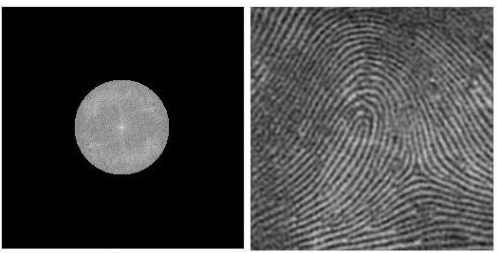
\includegraphics[scale=0.8]{Figure/figura1.PNG}
  \caption{Exemplo da aplicação do filtro passa-baixa.}
  \label{fig:figure1}
\end{figure}

\begin{figure}[!ht]
  \centering
  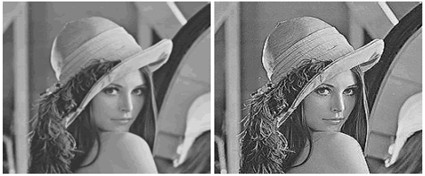
\includegraphics[scale=0.8]{Figure/figura2.jpg}
  \caption{Exemplo da aplicação do filtro passa-alta.}
  \label{fig:figure2}
\end{figure}

\subsubsection{Filtros não-lineares}
Os filtros não-lineares minimizam ruídos e suavizam bordas, alterando a média da imagem.
Eles alteram a imagem sem diminuir a sua resolução.
Há algumas técnicas como: 
\begin{itemize}
    \item Operadores para detecção de bordas: Detecta características, como bordas, linhas, curvas e manchas.
    Apresentando alguns exemplo de operadores:
    \begin{itemize}
        \item Operador de Roberts: 
        \begin{itemize}
            \item Denominado pela função: $$a'=\sqrt{(a-d)^2+(c-b)^2}$$
            \item Onde a' é o nível de cinza correspondente à localização a.
            $$\left[
            \begin{array}{c c c}
            a & b & \ldots\\
            c & d & \ldots\\
            \ldots & \ldots & \ldots\\
            \end{array}\right]$$
            \item Há o problema que algumas bordas podem ser mais realçadas que as outras dependendo da direção, mesmo possuindo a mesma magnitude.
        \end{itemize}
        \item Operador de Sobel:
        \begin{itemize}
            \item Mais sofisticado que o Operador de Roberts.
            \item Realça linhas verticais e horizontais mais escuras que o fundo, sem realçar pontos isolados.
            \item Utiliza duas máscaras:
            \begin{itemize}
                \item Máscara (a) = detecta as variações no sentido horizontal.
                $$\left[
                \begin{array}{c c c}
                -1 & 2 & -1\\
                0 & 0 & 0\\
                1 & 2 & 1\\
                \end{array}\right]$$
                \item Máscara (b) = detecta as variações no sentido vertical.
                $$\left[    
                \begin{array}{c c c}
                -1 & 0 & 1\\
                -2 & 0 & 2\\
                -1 & 0 & 1\\
                \end{array}\right]$$
                \item Em cada pixel, o resultado será dado pela equação: 
                $$a'= \sqrt{a^2+b^2}$$
                \item Onde a’ é o nível de cinza corresponde à localização do elemento central da máscara. 
                \end{itemize}
        \end{itemize}
    \end{itemize}
    \item Filtros morfológicos
    \begin{itemize}
        \item Exploram as propriedades geométricas dos sinais (níveis de cinza da imagem).  
        \item As máscaras são chamadas elementos estruturantes e os valores são 0 ou 1.
        \item Há 3 filtros morfológicos básicos:
        \begin{itemize}
            \item Filtro morfológico de mediana:
            \begin{itemize}
                \item Utilizado para suavização e eliminação de ruídos
                \item Mantém a dimensão da imagem.
            \end{itemize}
            \item Filtro morfológico de erosão:
            \begin{itemize}
                \item Provoca efeitos de erosão das partes claras da imagem (altos níveis de cinza), gerando imagens mais escuras.
            \end{itemize}
            \item Filtro morfológico de dilatação:
            \begin{itemize}
                \item Provoca efeitos de dilatação das partes escuras da imagem (baixos níveis de cinza), gerando imagens mais claras. 
            \end{itemize}
        \end{itemize}
    \end{itemize}
\end{itemize}

\begin{figure}[!ht]
    \centering
    
\includegraphics[scale=0.8]{Figure/figura4.PNG} 
    \caption{Exemplo da aplicação do operador de Roberts}
    \label{fig:figura4}
\end{figure}

\begin{figure}[!ht]
    \centering
    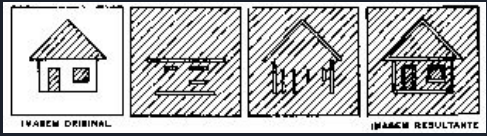
\includegraphics[scale=0.8]{Figure/figura3.PNG} 
    \caption{Exemplo da aplicação do operador de Sobel}
    \label{fig:figura3}
\end{figure}

A figura \ref{fig:figura4} mostra um exemplo de aplicação do Operador de Roberts e a figura \ref{fig:figura3} mostra um exeplo do operador de Sobel.

\par Para explicar os filtros morfológicos, assuma as seguintes matrizes como o elemento estruturante e a imagem.

Elemento estruturante:
$$\left[
    \begin{array}{c c c}
    0 & 1 & 0\\
    1 & 1 & 1\\
    0 & 1 & 0\\
    \end{array}\right]$$
    
Imagem:
$$\left[
    \begin{array}{c c c}
    3 & 6 & 5\\
    2 & 8 & 3\\
    2 & 6 & 5\\
    \end{array}\right]$$
    
No caso do filtro morfológico da mediana, o pixel central seria alterada para o valor 6 (valor mediano da sequência [2,3,6,6,8]).
No filtro morfológico de erosão, o valor central seria o menor valor da ordenação, sendo o valor 2 e no filtro morfológico de dilatação, o maior valor, sendo o valor 8.

\section{Detecção e correspondência de características}
\label{sec:detecção}
Nessa seção, será apresentado sobre características, detecção de características e alguns exemplos de detectores de características.
\subsection{Características e detecção de características}
Características são estruturas específicas em uma imagem. Cantos, arestas, curvas, podem ser exemplos de características.
\par Já detecção de características são métodos que detectam se para cada ponto de uma imagem existe uma informação de característica previamente abstraída.
Há diversos tipos de detecção de características:
\begin{itemize}
    \item Arestas: Canny, Sobel, Transformada de Hough
    \item Cantos: Operador de Harris
    \item Curvas
    \item Específicos por aplicação: k-curvatura
\end{itemize}

\subsection{Detector de características}
Será apresentado alguns exemplos de detector de características.
\subsubsection{Método de Canny}
O método de Canny é utilizado para a detecção de bordas. Diferente dos outros métodos de detecção de bordas, esse método possui dois refinamentos adicionais, detecta borda com largura de um pixel e fornece bordas fracas em regiões da imagem de menor contraste. 
O passo a passo do método de Canny é:
\begin{enumerate}
    \item Suavização da imagem com uma Gaussiana $G\sigma$
    \item Calcular o contraste da borda ($E_{s}$) é a magnitude do vetor gradiente, que é obtida dos gradientes vertical e horizontal da imagem, como nos outros métodos.
    \item Calcular a orientação da borda:
    O gradiente da imagem é um vetor composto por: $$\nabla I(x,y)=\frac{\partial I(x,y)}{\partial x}i + \frac{\partial I(x,y)}{\partial y}j $$
    \newline A orientação do vetor gradiente em cada pixel é obtida por:
    $$\theta(x,y) = \arctan\frac{\partial I(x,y)}{\partial y}/\frac{\partial I(x,y)}{\partial x}$$
    \item Eliminar pontos não-maximais da imagem de gradiente, calculando com as 4 direções ($0^\circ$, $45^\circ$, $90^\circ$ e $135^\circ$). Um pixel é contorno se a sua magnitude é máxima na direção do gradiente. 
    \item Limiarização com histerize: 
    \begin{enumerate}
        \item Definir dois limiares, $L_{baixo}$ e $L_{alto}$
        \item . Se um pixel da imagem $I_{N(i, j)} \le L_{alto}$ então marcar esse pixel como sendo uma borda
        \item Checar seus vizinhos na direção perpendicular ao gradiente $\theta(i, j)$. Se eles forem maiores do que $L_{baixo}$, então marcá-los como sendo bordas
    \end{enumerate} 
    Esse procedimento permite um limiar mais alto para eliminar ruídos ao mesmo tempo que não elimina bordas reais existentes na imagem.
\end{enumerate}

\subsubsection{Método de Sobel}
O método de Sobel é um operador que calcula diferenças finitas, dando uma aproximação do gradiente da intensidade dos pixels da imagem. 
\par Em cada ponto da imagem, o resultado da aplicação do filtro Sobel devolve o gradiente da intensidade em cada ponto, dando a direção da maior variação de claro para escuro e a quantidade de variação nessa direção, obtendo uma noção de como varia a luminosidade em cada ponto.
\par Sendo A a imagem inicial então, $G_{x}$ e $G_{y}$ serão duas imagens que em cada ponto contém uma aproximação às derivadas horizontal e vertical de A:
$$G_{x}= \left[
    \begin{array}{c c c}
    -1 & 0 & 1\\
    -2 & 0 & 2\\
    -1 & 0 & 1\\
    \end{array}\right]* A$$
$$G_{y}= \left[
    \begin{array}{c c c}
     1 & 2 & 1\\
     0 & 0 & 0\\
    -1 & -2 & -1\\
    \end{array}\right]*A$$

A  magnitude G e a direção do gradiente $\theta$ são obtidas por:
$$G=\sqrt{G_{x}^2+G_{y}^2}$$
$$\theta=\arctan(\frac{G_{y}}{G_{x}})$$

\subsubsection{SIFT (\textit{Scale Invariant Feature Transform)})}
O SIFT é uma técnica de processamento de imagens que permite a detecção e extração de descritores locais. Ele não varia em mudanças de iluminação, ruídos, rotação, escala.
De forma simplificada, as 4 etapas são:
\begin{enumerate}
    \item Detecção dos máximos locais = \textit{Keypoints}
    \item Localização dos \textit{keypoints} = Refinamento
    \item Cálculo da orientação dos \textit{keypoints} considerando o gradiente = Invariante à rotação
    \item Gera descritor de acordo com orientação do \textit{keypoint}
\end{enumerate}

\section{Texturas}
\label{sec:texturas}
Texturas são facilmente perceptíveis pela visão humana, mas pela visão computacional é uma tarefa complexa. 
\par As texturas contém diversas informações. Entre elas há informações sobre a distribuição espacial, variação de luminosidade, suavidade, rugosidade, regularidade e além disso, descreve o arranjo estrutural das superfícies e as relações vizinha.
\par As texturas podem ser aplicadas em:

\begin{itemize}
    \item Segmentação ou divisão de uma imagem em regiões
    \item Descrição de regiões
    \item Classificação se rotulação de uma região
    \item Análise de forma
    \item Réplica para caracterizar superfícies (síntese de imagens)
\end{itemize}

\subsection{Identificação de texturas}
Há diversas maneiras de identificar as texturas:
\begin{itemize}
    \item Entropia de uma imagem: Quantidade de cada um dos $aj$ tons (histograma) ou $aj$ texturas.
    $$H(Pa)=\sum_{i=1}^{J} p(a_{j})logp(a_{j})$$
    \item Coeficiente de Hurst: Aproximação da DF(dimensão fractal) para imagens. 
    $$D=\frac{lnN}{ln(1/r)}$$
    N = Quantidade de partes que a imagem foi dividida, r = fator de escala
    \item Coeficientes de variação espacial: Medida de dispersão (coeficiente de variação) do conjunto de pixels pertencentes à região da imagem.
    $$CV=\frac{DP}{\bar{x}}*100$$
    $$\bar{x}=\frac{\sum_{i=1}^{n} xi}{n}$$
    $\bar{x}$=medida de posição (média)
    \item Outros
    \begin{itemize}
        \item Dimensão Fractal
        \item Momentos de Intensidades
        \item Matrizes de Co-ocorrência
        \item Descritores de Textura de Haralick
        \item Funções de Autocorrelação
        \item LZW
        \item Matriz de comprimentos corridos
        \item Spatiograms
        \item Descritores de Textura baseados nos Histogramas de Soma e Diferenças ...
    \end{itemize}
\end{itemize}

\subsection{Análise de textura}
Há dois tipos de análise, a análise estrutural e a análise estatística.

\subsubsection{Análise estrutural}
A análise é baseada em repetição dos padrões primitivos básicos com uma certa regra de posicionamento.
Não são muitos aplicados, pois as texturas mais comuns não são tão regulares para utilizar esse método.

\subsubsection{Análise estatística}
Há dois tipos:
\begin{itemize}
    \item Primeira ordem:
    \begin{itemize}
        \item Define com que frequência um pixel aparece na imagem
        \item Depende somente de valores de pixel individuais e não de interação ou co-ocorrência de pixels vizinhos, não levando em consideração a distribuição espacial dos níveis de cinza da imagem.
        \item Exemplo: média, variância, desvio padrão, simetria, energia, entropia...
    \end{itemize}
    \item Segunda ordem:
    \begin{itemize}
        \item Observação de um par de pixels, em uma distância randômica numa imagem, numa orientação e posição randômica
        \item Obtém um resultado mais preciso, pois leva o posicionamento em consideração
        \item Exemplo: SGLDM - \textit{Spatial Grey Level Dependence Level}, GLDM - \textit{Grey Level Difference Method}, RLM - \textit{Run
        Length Method}
    \end{itemize}
\end{itemize}

\begin{figure}[!ht]
    \centering
    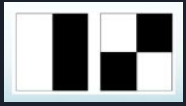
\includegraphics[scale=0.8]{Figure/figura5.PNG}
    \caption{Análise estatística de primeira ordem e segunda ordem}
    \label{fig:figura5}
\end{figure}

A principal diferença entre essas duas análises é que a segunda leva em consideração a posição dos pixels. Isso significa que se a análise de primeira ordem analisasse os dois casos da figura \ref{fig:figura5}, os histogramas dos dois casos seriam iguais, mas a análise de segunda ordem resultaria em diferentes histogramas.

\subsection{Exemplo de medidas de análise}
\begin{itemize}
    \item Primeira ordem:
    \begin{itemize}
        \item n-ésimo momento do histograma de uma imagem:
        $$ \mu _{n}(z)=\sum_{i=1}^{L} (z_{i}-m)^n p(z_{i})$$
        $$m=\sum_{i=1}^{L}z_{i}p(z_{i})$$
    \end{itemize}
    
    \item Suavidade relativa R da textura
    $$R=1-\frac{1}{1+\omega^2(z)}$$
    
    \item Obliquidade (\textit{skewness})
    $$V=\frac{\mu_{3}}{\omega^3}$$
    
    \item Curtose (achamento da distribuição)
    $$K=\frac{\mu_{4}}{\omega^4(z)}-3$$
    
    \item Segunda ordem
    \begin{itemize}
        \item Matrizes de co-ocorrência(Matriz de ocorrência simultânea)
    
        \begin{itemize}
            \item Faz uma relação entre dois pixels por vez, um chamado de pixel referência e o outro de pixel vizinho
            \item Representa a distância e as relações espaciais angulares sobre uma sub-região de uma imagem de tamanho especificado
            \item Cada elemento da matriz é uma medida de probabilidade de ocorrência de valores de níveis de cinza separados por uma dada distância numa dada direção 
            \item A matriz de co-ocorrência de uma imagem I quantizada em N níveis de cinzas para dado um ângulo e uma distância é representada por uma matriz M onde M(p, q) indica a quantidade de ocorrências onde um pixel de intensidade q é vizinho de um pixel de intensidade p a uma distância e formando um ângulo X com o mesmo
        \end{itemize}
        
        \begin{figure}[!ht]
            \centering
            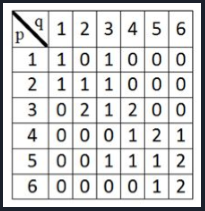
\includegraphics[scale=0.8]{Figure/figura6.PNG}
            \caption{Exemplo de Matriz de ocorrência}
            \label{fig:figure6}
        \end{figure}
        
        \item Matrizes Run-Length
        \begin{itemize}
            \item Codifica a textura levando em consideração a quantidade de vezes que um mesmo nível de cinza i aparece em uma sequência j a uma determinada direção
            \item Produz medidas baseado no número de sequências de tons de cinza para um certo comprimento (\textit{Run length})
            \item A sequência forma conjunto de pixels consecutivos e co-lineares com a mesma intensidade
        \end{itemize}
        
        \begin{figure}[!ht]
            \centering
            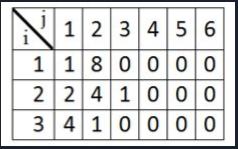
\includegraphics[scale=0.8]{Figure/figura7.PNG}
            \caption{Exemplo de Matriz Run Length}
            \label{fig:figure7}
        \end{figure}
        
    \end{itemize}
    
\end{itemize}

\section{Segmentação de imagens}
\label{sec:segmentação}
A segmentação de uma Imagem I é uma partição em regiões homogêneas R1, R2, …., Rn tal que:
\begin{enumerate}
    \item Todo pixel pertence a uma região $I=\bigcup_{i=1}^nR_{i}$
    \item $R_{i}$ é uma região conexa para todo $i=1,2,...,n$
    \item Nenhum pixel pertence a mais de uma região \\
    $R_{i}\cap R_{j}=\varnothing, \forall i \neq j$
\end{enumerate}

\subsection{Estratégias de segmentção}
Há dois tipos de estratégias:
\begin{itemize}
    \item Descontinuidade dos níveis de cinza
    \begin{itemize}
        \item A partição da imagem é feita com as alterações bruscas de intensidade 
        \item Exemplo: Detecção de linhas, bordas, pontos isolados
    \end{itemize}
    \item  Similaridade dos níveis de cinza 
    \begin{itemize}
        \item A partição da imagem é feita através da similaridade dos pixels, seguindo um critério
        \item Exemplo: Binarização, crescimento de regiões, divisão, junção de regiões
    \end{itemize} 
\end{itemize}

\subsubsection{Detecção de descontinuidades}
Procura por pontos isolados.
\begin{itemize}
    \item Detecção de linhas: Feita através do uso de um filtro passa altas direcionais 
    \item Detecção de contornos
    \begin{itemize}
        \item Mais utilizado entre os métodos de detecção de descontinuidades
        \item Geralmente efetuada a partir do cálculo da primeira e da segunda derivada da imagem 
        \item Bordas = normalmente são borradas 
        \item Existência de imperfeições no processo de aquisição da imagem podem causar “rampas” no contorno da imagem 
        \item A magnitude da primeira derivada e as passagens por zero da segunda derivada podem ser utilizadas para detectar os contornos
    \end{itemize}
\end{itemize}

\subsubsection{Detecção de similaridade}
Procura por pontos semelhantes.

\begin{itemize}
    \item Limiarização
    \begin{itemize}
        \item Consiste em separar regiões de uma imagem quando esta apresenta fundo se objeto (\textit{background}, \textit{foreground}) 
        \item Extrai objetos selecionando um limiar T que separa o fundo e o objeto
        \item Há 3 tipos de limiares: 
        \begin{itemize}
            \item Global:
            \begin{itemize}
                \item Para cada ponto $(s,y)$ tal que $f(s,y) > T$ denominado ponto do objeto, caso contrário fundo 
                \item  $$g(x,y) = \left \{ \begin{matrix} 1, & \mbox{se }f(x,y)>L \mbox{(forma)} \\ 0, & \mbox{se }f(x,y) \le L \mbox{(fundo)} \end{matrix} \right.$$
                \item  Depende apenas de f(x,y)
            \end{itemize}
            \item Adaptativo:
            \begin{itemize}
                \item  Seleciona um limiar individual para cada pixel baseado no alcance da intensidade estimado em sua vizinhança local
                \item Melhor limiarização quando não existem cumes bem definidos
                \item  Passo a passo: 
                    \begin{enumerate}
                        \item Dividir a imagem original em sub-imagens 
                        \item Determinar um limiar independentemente para cada região 
                        \item Cada imagem $R_{i}$ é então processada usando um limiar local
                        \item Uma nova imagem $R'$ é definida por $R' = U * Ri$
                    \end{enumerate}  
            \end{itemize}
            \item Local:
            \begin{itemize}
                \item Semelhante ao global, mas utiliza propriedades locais 
                \item Além das intensidades, utiliza-se uma propriedade local
                \item $T(x,y)  = T(l(x,y), P(x,y))$
            \end{itemize}
        \end{itemize}
    \end{itemize}
\end{itemize}

Um bom limiar é aquele que causa um erro mínimo. \\ Ele pode ser achado pelos seguintes métodos:

\begin{itemize}
    \item Valor obtido por testes 
    \item Valor médio dos tons de cinza 
    \item Valor mediano entre o tom máximo e o tom mínimo 
    \item Algoritmos automáticos (Otsu, Kittler...)
\end{itemize}

\subsubsection{Algoritmos de limiarização de Otsu}
Permite a seleção automática do valor do limiar T.
Passo a passo do algoritmo:
\begin{enumerate}
    \item  Normalizar o histograma de acordo com: 
    $$p_{r}(r_{k})=\frac{n_{k}}{n}$$ \\
    Onde:
    \begin{itemize}
        \item $0 \le r_{k} \le 1 \mbox{ e } k = 0,1,2, \ldots L-1$
        \item L = número de níveis de cinza da imagem 
        \item n = número total na imagem
        \item $p_{r}(r_{k})$ = percentual do k-ésimo nível de cinza
        \item $n_{k}$ = número de pixels cujo nível de cinza corresponde k 
    \end{itemize}
    \item  Para um determinado limiar T, têm-se dois grupos de pixels
    \begin{itemize}
        \item Grupo C0 formado pelos valores {0,1,2, …., T-1} 
        \item Grupo C1 formado pelos valores {T, T+1, …, L}
    \end{itemize}
    \item Encontrar a variância 
    $$\sigma_{B}^2=w_{0}(\mu_{0}-\mu_{T})^2+w_{1}(\mu_{1}-\mu_{T})^2$$
    Onde:
    \begin{itemize}
        \item $w_{0}$ = probabilidade de c0 
        \item $w_{1}$ = probabilidade de c1 
        \item $\mu_{0}$ = média de c0
        \item $\mu_{1}$ = média de c1
        \item $\mu_{T}$ = média total
        \item $k$ = nível de cinza
    \end{itemize}
    \item Aplicar a equação da variância para todos possíveis limiares e escolher o de maior valor
\end{enumerate}

\section{References}
\small
\begin{itemize}
    \item Material da Divisão de Processamento de Imagens (DPI), Teoria: Processamento de Imagens, disponível em: \url{http://www.dpi.inpe.br/spring/teoria/filtrage/filtragem.htm}
    \item Material do Professor Eduardo L.L. Cabral, disponível em: \url{https://edisciplinas.usp.br/pluginfile.php/4112482/mod_resource/content/0/V10%20-Deteccao%20de%20bordas.pdf}
    \item Material do Departamento de Informática da PUC-RJ, Trabalho de Imagem, disponível em: \url{http://www.inf.puc-rio.br/~asouza/FCG/imagem.html}
    \item Material do Professor Kamel Bensebaa, disponível em: \url{http://slideplayer.com.br/slide/10104678/}
\end{itemize}

\end{document}
